

\tikzset{every picture/.style={line width=0.75pt}} %set default line width to 0.75pt        
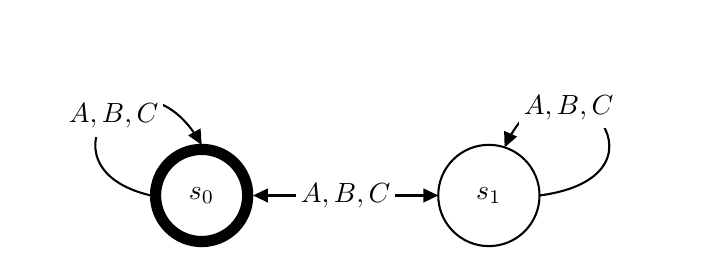
\begin{tikzpicture}[x=0.75pt,y=0.75pt,yscale=-0.8,xscale=0.8]
%uncomment if require: \path (0,150); %set diagram left start at 0, and has height of 150

%Shape: Circle [id:dp4325934269433842] 
\draw  [fill={rgb, 255:red, 0; green, 0; blue, 0 }  ,fill opacity=1 ] (216.5,93) .. controls (216.5,76.16) and (230.16,62.5) .. (247,62.5) .. controls (263.84,62.5) and (277.5,76.16) .. (277.5,93) .. controls (277.5,109.84) and (263.84,123.5) .. (247,123.5) .. controls (230.16,123.5) and (216.5,109.84) .. (216.5,93) -- cycle ;
%Shape: Circle [id:dp8959340303758652] 
\draw   (389.5,93) .. controls (389.5,76.16) and (403.16,62.5) .. (420,62.5) .. controls (436.84,62.5) and (450.5,76.16) .. (450.5,93) .. controls (450.5,109.84) and (436.84,123.5) .. (420,123.5) .. controls (403.16,123.5) and (389.5,109.84) .. (389.5,93) -- cycle ;
%Straight Lines [id:da6159546739572547] 
\draw    (280,93) -- (387.5,93) ;
\draw [shift={(389.5,93)}, rotate = 180] [fill={rgb, 255:red, 0; green, 0; blue, 0 }  ][line width=0.75]  [draw opacity=0] (8.93,-4.29) -- (0,0) -- (8.93,4.29) -- cycle    ;
\draw [shift={(278,93)}, rotate = 0] [fill={rgb, 255:red, 0; green, 0; blue, 0 }  ][line width=0.75]  [draw opacity=0] (8.93,-4.29) -- (0,0) -- (8.93,4.29) -- cycle    ;
%Curve Lines [id:da8452234444075793] 
\draw    (216.5,93) .. controls (142.87,76.08) and (207.84,-5.18) .. (246.42,61.48) ;
\draw [shift={(247,62.5)}, rotate = 240.66] [fill={rgb, 255:red, 0; green, 0; blue, 0 }  ][line width=0.75]  [draw opacity=0] (8.93,-4.29) -- (0,0) -- (8.93,4.29) -- cycle    ;

%Curve Lines [id:da8370233876099651] 
\draw    (450.5,93) .. controls (540.91,81.08) and (462.16,-7.43) .. (429.98,62.93) ;
\draw [shift={(429.5,64)}, rotate = 293.78] [fill={rgb, 255:red, 0; green, 0; blue, 0 }  ][line width=0.75]  [draw opacity=0] (8.93,-4.29) -- (0,0) -- (8.93,4.29) -- cycle    ;

%Shape: Circle [id:dp08152116050102409] 
\draw  [fill={rgb, 255:red, 255; green, 255; blue, 255 }  ,fill opacity=1 ] (222,93) .. controls (222,79.19) and (233.19,68) .. (247,68) .. controls (260.81,68) and (272,79.19) .. (272,93) .. controls (272,106.81) and (260.81,118) .. (247,118) .. controls (233.19,118) and (222,106.81) .. (222,93) -- cycle ;

% Text Node
\draw  [color={rgb, 255:red, 255; green, 255; blue, 255 }  ,draw opacity=1 ][fill={rgb, 255:red, 255; green, 255; blue, 255 }  ,fill opacity=1 ]  (304.75,81) -- (362.75,81) -- (362.75,105) -- (304.75,105) -- cycle  ;
\draw (333.75,93) node   {$\agent{A}, \agent{B}, \agent{C}$};
% Text Node
\draw (247,93) node   {$\defemph{s_0}$};
% Text Node
\draw (420,93) node   {$\defemph{s_1}$};
% Text Node
\draw  [color={rgb, 255:red, 255; green, 255; blue, 255 }  ,draw opacity=1 ][fill={rgb, 255:red, 255; green, 255; blue, 255 }  ,fill opacity=1 ]  (165,33) -- (223,33) -- (223,57) -- (165,57) -- cycle  ;
\draw (194,45) node   {$\agent{A}, \agent{B}, \agent{C}$};
% Text Node
\draw  [color={rgb, 255:red, 255; green, 255; blue, 255 }  ,draw opacity=1 ][fill={rgb, 255:red, 255; green, 255; blue, 255 }  ,fill opacity=1 ]  (439,28) -- (497,28) -- (497,52) -- (439,52) -- cycle  ;
\draw (468,40) node   {$\agent{A}, \agent{B}, \agent{C}$};

%\draw (340,160) node   {%
%	$\begin{aligned}
%	\interp{0}{s_0}&=\bra{\looking {AG}, \haskey A}\\
%	\interp{0}{s_1}&=\bra{\looking {AG}, \haskey{A}, \head}
%	\end{aligned}$
%	\hspace*{0.2cm}where \agent{ag} $\in$ \bra{\agent{a}, \agent{b}, \agent{c}}.};

\end{tikzpicture}

